\noindent
\begin{minipage}[t]{0.27\textwidth}
  \vspace{0pt}% Khóa đỉnh tọa độ minipage
  \vspace{2.2cm}% Dóng ngang với hàng 10^3 = 1000 trong bản gốc
  \noindent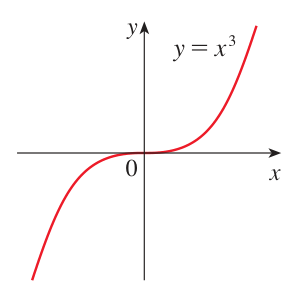
\includegraphics[width=\linewidth]{images/p0168_fig1.png}
  
  \vspace{1mm}
  \noindent{\small\textbf{\textsf{HÌNH 11}}}\\[2pt]
  {\footnotesize $\lim\limits_{x \to \infty} x^3 = \infty,\;\lim\limits_{x \to -\infty} x^3 = -\infty$}

  \vspace{0.8cm}% Dóng ngang với đoạn thảo luận Hình 10 & 12
  \noindent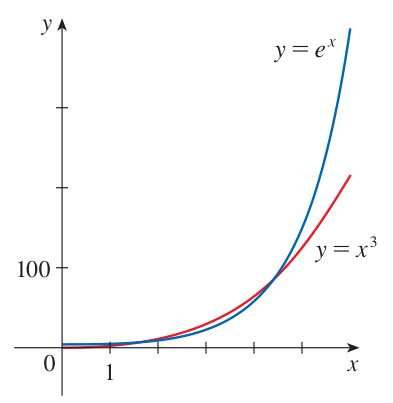
\includegraphics[width=\linewidth]{images/p0168_fig2.png}
  
  \vspace{1mm}
  \noindent{\small\textbf{\textsf{HÌNH 12}}}\hspace{0.5em}{\footnotesize $e^x$ lớn hơn $x^3$ rất nhiều khi $x$ lớn.}
\end{minipage}%
\hfill
\begin{minipage}[t]{0.70\textwidth}
  \vspace{0pt}% Khóa đỉnh tọa độ minipage
  \setlength{\parindent}{0pt}
  \setlength{\parskip}{0pt}

  \noindent\textbf{\textsf{\color{stewartcyan}VÍ DỤ 9}}\hspace{1.2em}Tìm $\lim\limits_{x \to \infty} x^3$ và $\lim\limits_{x \to -\infty} x^3$.

  \medskip
  \noindent\textbf{\textsf{\color{stewartcyan}LỜI GIẢI}}\hspace{1.2em}Khi $x$ trở nên lớn, $x^3$ cũng trở nên lớn. Chẳng hạn,
  \[
  10^3 = 1000 \qquad\quad 100^3 = 1{,}000{,}000 \qquad\quad 1000^3 = 1{,}000{,}000{,}000
  \]
  Trên thực tế, ta có thể làm cho $x^3$ lớn tùy ý bằng cách yêu cầu $x$ đủ lớn. Do đó ta có thể viết
  \[
  \lim_{x \to \infty} x^3 = \infty
  \]
  Tương tự, khi $x$ là số âm có giá trị tuyệt đối lớn, $x^3$ cũng vậy. Do đó
  \[
  \lim_{x \to -\infty} x^3 = -\infty
  \]
  Các khẳng định giới hạn này cũng có thể thấy được từ đồ thị của hàm số $y = x^3$ trong Hình~11.\hfill\stewartbox

  \vspace{1em}
  Quan sát Hình~10 ta thấy rằng
  \[
  \lim_{x \to \infty} e^x = \infty
  \]
  nhưng, như Hình~12 minh họa, $y = e^x$ trở nên rất lớn khi $x \to \infty$ với tốc độ nhanh hơn nhiều so với $y = x^3$.

  \vspace{1.2em}
  \noindent\textbf{\textsf{\color{stewartcyan}VÍ DỤ 10}}\hspace{1.2em}Tìm $\lim\limits_{x \to \infty} (x^2 - x)$.

  \medskip
  \noindent\textbf{\textsf{\color{stewartcyan}LỜI GIẢI}}\hspace{1.2em}Quy tắc Giới hạn 2 nói rằng giới hạn của một hiệu bằng hiệu các giới hạn, với điều kiện các giới hạn này tồn tại. Chúng ta không thể sử dụng Quy tắc 2 ở đây vì
  \[
  \lim_{x \to \infty} x^2 = \infty \qquad \text{và} \qquad \lim_{x \to \infty} x = \infty
  \]
  \warningicon\hspace{0.5em}Nói chung, \textcolor{stewartred}{các Quy tắc Giới hạn không thể áp dụng cho các giới hạn vô cực} vì $\infty$ không phải là một số ($\infty - \infty$ không thể xác định được). Tuy nhiên, chúng ta \emph{có thể} viết
  \[
  \lim_{x \to \infty} (x^2 - x) = \lim_{x \to \infty} x(x - 1) = \infty
  \]
  vì cả $x$ và $x - 1$ đều trở nên lớn tùy ý và do đó tích của chúng cũng vậy.\hfill\stewartbox

  \vspace{1.2em}
  \noindent\textbf{\textsf{\color{stewartcyan}VÍ DỤ 11}}\hspace{1.2em}Tìm $\lim\limits_{x \to \infty} \dfrac{x^2 + x}{3 - x}$.

  \medskip
  \noindent\textbf{\textsf{\color{stewartcyan}LỜI GIẢI}}\hspace{1.2em}Như trong Ví dụ~3, ta chia cả tử thức và mẫu thức cho lũy thừa bậc cao nhất của $x$ ở mẫu thức, ở đây đơn giản chính là $x$:
  \[
  \lim_{x \to \infty} \frac{x^2 + x}{3 - x} = \lim_{x \to \infty} \frac{x + 1}{\dfrac{3}{x} - 1} = -\infty
  \]
  vì $x + 1 \to \infty$ và $3/x - 1 \to 0 - 1 = -1$ khi $x \to \infty$.\hfill\stewartbox
\end{minipage}
